\section{Technical Implementation and Details}

\subsection{FIDO2}

As already briefly introduced in \autoref{subsec:fido_alliance}, the \gls{fido}2 project is a joint efforts of the \gls{w3c} and the \gls{fido} alliance. It consists of the JavaScript standard, the \wa{}, and the \gls{ctap}. The \wa{} is standardized and managed by the \gls{w3c}, while the \gls{ctap} is authored by the \gls{fido} alliance. However, the \gls{fido} alliance also initially developed the \wa{} under the name \gls{fido} 2.0 before officially handing it over to the \gls{w3c}.\footcites[See][254]{Schwartz2018}[See][3]{FormalVerificationWebAuthn}

\begin{figure}[hbt]
	\centering
	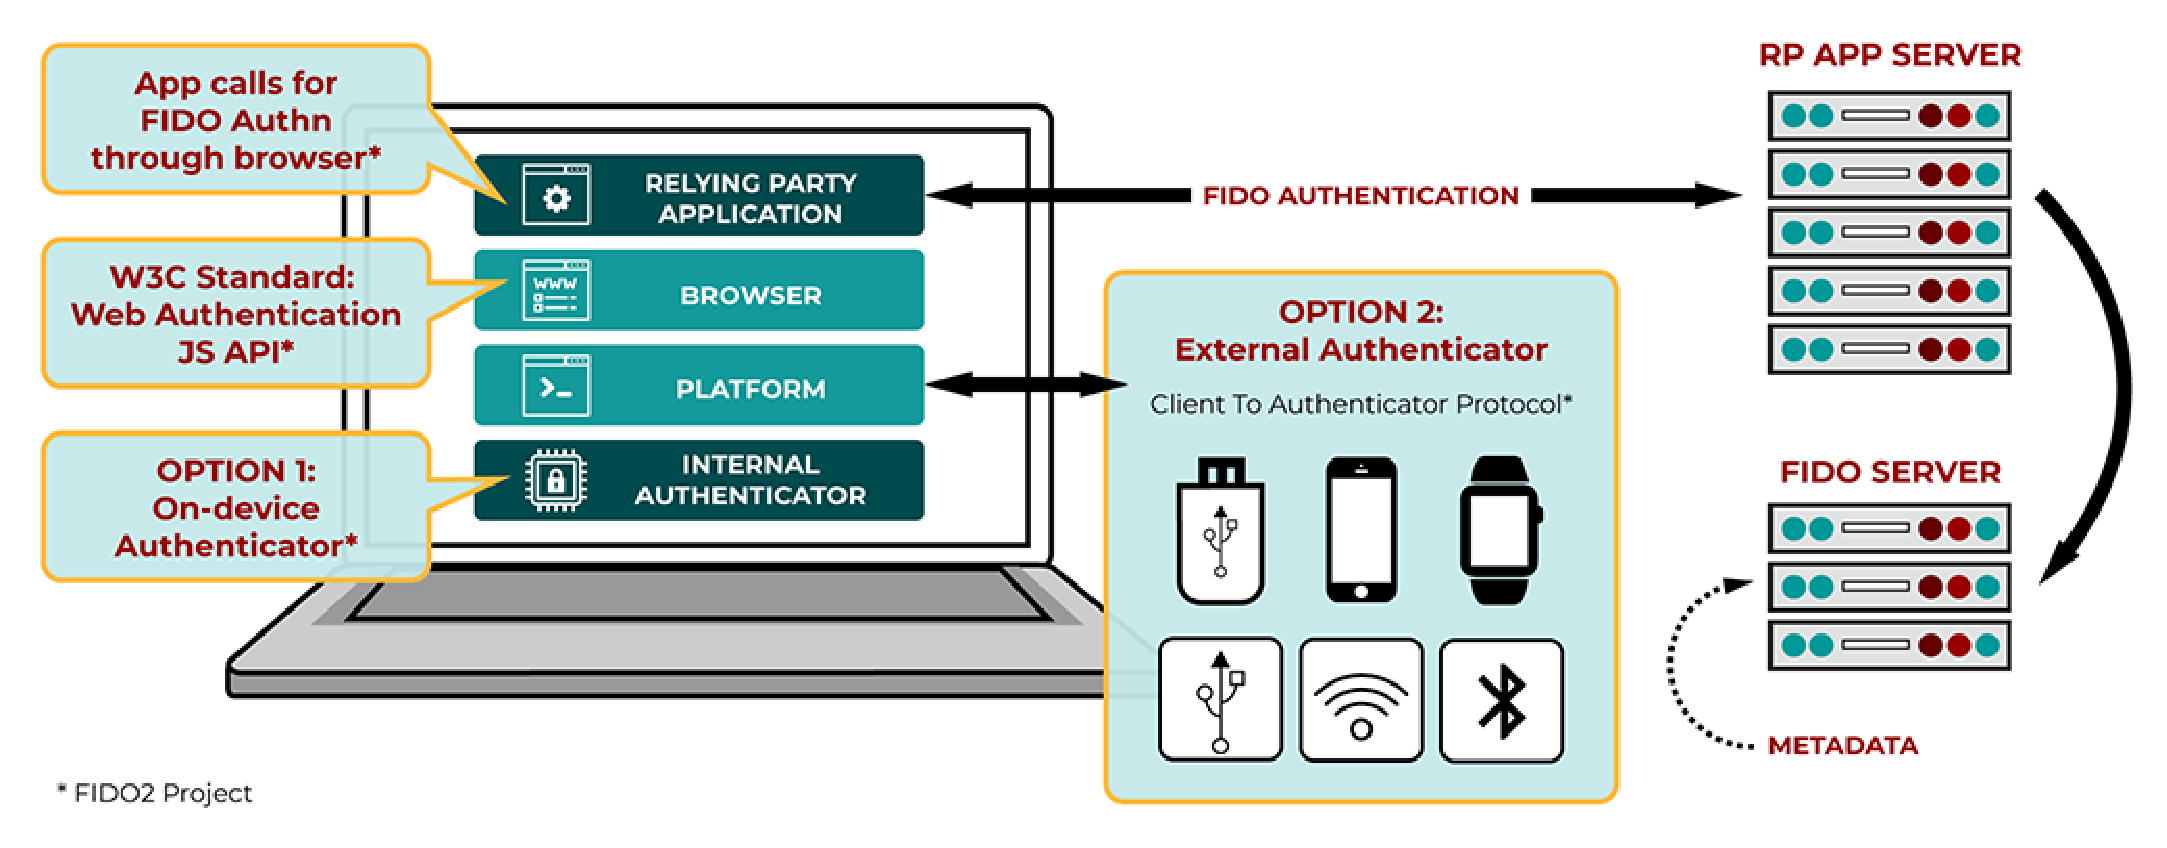
\includegraphics[width=\textwidth]{pics/FIDO2-Graphic-v2.eps}
	\caption[\gls{fido}2 architecture overview]{\gls{fido}2 architecture overview\footnotemark}
	\label{fig:fido2_architecture}
\end{figure}
\footnotetext{Source: https://fidoalliance.org/specifications/, last access on 09/14/2019}

\autoref{fig:fido2_architecture} shows the overview of the \gls{fido}2 project. A noteworthy change is the possibility to use either a \textit{roaming}, i.e., external authenticator or an authenticator that is built into the device.

\subsection{Client to Authenticator Protocol 2}

The \glsfirst{ctap} 2 is based on the \gls{u2f} protocol version 1.2 and defines three parts:

\begin{enumerate}
	\item the authenticator \gls{api}
	\item message encoding
	\item transport-specifc binding
\end{enumerate}

The key methods of the authenticator \gls{api} are explained in more detail below. Message encoding describes the process of encoding the corresponding message in a binary encoding called \gls{cbor} that is suitable for, e.g., the transport over \gls{ble}, because plain text string and \gls{json} objects can be too big for a transport over such protocols. The transport-specific bindings define the required transformation and bindings in order to comply with the transport protocol specifications.\footcites[See][4--5]{ctap2}

An important difference between \gls{ctap}2 and the preceding standard \gls{u2f} is the fact that \gls{ctap}2 describes only the communication between the client, i.e., web browser and the authenticator, as opposed to \gls{u2f} where the standard also defines the JavaScript \gls{api} in order to communicate with the authenticator. \autoref{fig:ctap_vs_u2f} shows this architectural difference.\footcites[See][51]{kim-new-way-fido}[See][254]{Schwartz2018}

\begin{figure}[hbt]
	\centering
	\includesvg[width=\textwidth,pretex=\relscale{0.8}]{pics/svg/ctap_vs_u2f}
	\caption[Architectural differences of \gls{u2f} and \gls{ctap}2]{Architectural differences of \gls{u2f} and \gls{ctap}2\footnotemark}
	\label{fig:ctap_vs_u2f}
\end{figure}
\footcitetexts[Source: diagram by author, based on][4]{u2f-overview}[][Chapter 6]{w3c}

\subsubsection{Registration}

The registration procedure calls the method \textit{authenticatorMakeCredential}. The input parameters are identical to the ones defined in the higher level \wa{} and are further explained in \autoref{subsec:wa}. Upon reception of the required data, the authenticator first checks if the \textit{excludeList} if a credential ID is listed that is already registered on the authenticator. This prevents that a user registers multiple accounts. If the user verification or presence option is passed, the authenticator has to ensure a legitimate user is present. Upon successful user verification the authenticator generates a new credential key-pair for the specified algorithm.\footcites[See][9]{ctap2}

After that, the authenticator generates the attestation object consisting of the authentication data, which contain the hash of the \gls{rp} ID, a counter, flags if the user has been verified, and the public key with its unique credential ID. Besides that, the authenticator also sends the attestation statement if required. This statement can for example be issued by the \gls{tpm}, Android Key attestation, or the private attestation key of the authenticator token.\footcites[See][9]{ctap2}[See][Chapter 8]{w3c}

\subsubsection{Authentication and transaction confirmation}

Authentication is performed by using the method \textit{authenticatorGetAssertion} of the \gls{ctap} protocol. Again the higher level \wa{} defines the input parameters. The identifier of the \gls{rp} is sent to the authenticator and optionally a list of allowed public keys the authenticator is allowed to retrieve. After optional user verification and presence detection the authenticator displays the data to the user if it has a display to do so. When these checks succeeded, the authenticator accesses the corresponding credentials.\footcites[See][11-13]{ctap2}

The authenticator generates an assertion signature over the received hash of the client data and the authenticator data which consist of the hashed \gls{rp} ID, the flags for user presence and verification, a counter, and the attested credential data. The attested credential data comprises of the \gls{aaguid}, credential ID and the credential public key.\footcites[See][Chapter 6.4.1.]{w3c}

\subsubsection{Factory reset}

As the \gls{uaf} protocol, but in contrast to the \gls{u2f} specification, the \gls{ctap} does define a method to completely factory reset the authenticator in order to de-register every user account on it. To avoid accidental deletion of all user accounts, the protocol specifies that the authenticator may ask for user confirmation. However, it is not possible to delete a specific user account.\footcites[See][26]{ctap2}

\subsection{Web Authentication API}
\label{subsec:wa}

The API defined in the WebAuth is actually an extension of the Credential Management API, which is another API in development, but currently in a draft state. The Credential Management API defines \textit{navigator.credentials} property with the \textit{create} and \textit{get} methods and has the goal to offer an API for programatically accessing the user agent's password storage capabilities. The \wa{} is adding further method overloads to support public-key based credentials, too.

The \wa{} is backwards compatible to the \gls{u2f} compatible, thus making every security token that is usable for \gls{u2f} compatible with the \wa, too. However, a crucial restriction of the legacy \gls{u2f} protocol in usage with \gls{fido}2 is, that it is only usable as a second factor and not for passwordless logins.

\subsubsection{Registration}

\begin{example}{Exemplary Web Authentication API registration}{listing:webauthnreg}
\begin{minted}[breaklines]{javascript}
const publicKeyOptions = {
  challenge: 'Wings2019', // normally random string from the server in binary form (Uint8Array)
  rp: {
    name: 'Web Authn Test',
    id: 'https://timbrust.de'
  },
  user: {
    id: 'C0E3F2BFCFA8179F', // usually in binary form (Uint8Array)
    name: 'me@timbrust.de',
    displayName: 'tim'
  },
  pubKeyCredParams: [{ alg: -7, type: 'public-key' }],
  authenticatorSelection: {
    authenticatorAttachment: 'cross-platform'
  },
  timeout: 600,
  attestation: 'none'
};

const credential = await navigator.credentials.create({
  publicKey: publicKeyOptions
});
\end{minted}
\end{example}

\autoref{listing:webauthnreg} shows an example payload for the registration of a new credential with the \wa. Noteworthy parameter and options include the \textit{user.id}, which should not be an information that could lead to user identification because this ID can be stored on the authenticator.

\begin{example}{Web Authentication API registration response}{listing:webauthnregresp}
\begin{minted}[breaklines]{javascript}
const credential = {
  id: 'BShOCQ2c32dv4aqyy3oWmcu_9s4tz0VIob81U5tg [...]',
  rawId: ArrayBuffer(59),
  response: {
    clientDataJSON: ArrayBuffer(121),
    attestationObject: ArrayBuffer(306)
  },
  type: 'public-key'
};
\end{minted}
\end{example}

\autoref{listing:webauthnregresp} shows the received response from the creation generation, i.e., the newly generated credentials for the \gls{rp}.

\begin{example}{Web Authentication API registration client data}{listing:webauthnregrespclientdata}
\begin{minted}[breaklines]{javascript}
const clientDataJSON = {
  challenge: 'Wings2019',
  origin: 'https://timbrust.de',
  type: 'webauthn.create'
};
\end{minted}
\end{example}

\autoref{listing:webauthnregrespclientdata} shows the decoded client data from the \wa{} registration response from \autoref{listing:webauthnreg}. The data contains the challenge sent by the \gls{rp} and the origin of the \gls{rp}. Each registration is flagged with the type of \texttt{webauthn.create}.

\begin{example}{Web Authentication API registration attestation}{listing:webauthnregrespattestation}
\begin{minted}[breaklines]{javascript}
const attestationObject = {
  fmt: 'fido-u2f',
  attStmt: {
    sig: '[...]',
    x5c: []
  },
  authData: {
    rpIdHash: '068a7ad7f858dadbf691af6f2f7ca86d4dee5a080b [...]',
    flags: {
      userPresent: true,
      reserved1: false,
      userVerified: false,
      reserved2: '0',
      attestedCredentialData: true,
      extensionDataIncluded: false
    },
    signCount: 0,
    attestedCredentialData: {
      aaguid: '0000000000000000',
      credentialIdLength: 96,
      credentialId: ArrayBuffer(59), // same as publicKeyCredential.id
      credentialPublicKey: {
        kty: 'EC',
        alg: 'ECDSA_w_SHA256',
        crv: 'P-256',
        x: 'xHxgcBFgJolQ5lvukADki+cUzTPcmk50tfj0YGH3nYE=',
        y: 'W1OKIxfc6pIE/ANeTD7MqnNVjBXd0L7We9xZ3Hx6nD8='
      }
    }
  }
};
\end{minted}
\end{example}

\subsubsection{Authentication}

\begin{example}{Exemplary Web Authentication API authentication}{listing:webauthnauth}
\begin{minted}[breaklines]{javascript}
const publicKeyOptions = {
  challenge: 'Wings2019Auth', // normally random string from the server in binary form (Uint8Array)
  allowCredentials: [
    {
      id: 'BShOCQ2c32dv4aqyy3oWmcu_9s4tz0VIob81U5tg [...]',
      type: 'public-key',
      transports: ['usb', 'ble', 'nfc']
    }
  ],
  timeout: 6000
};

const assertion = await navigator.credentials.get({
  publicKey: publicKeyOptions
});
\end{minted}
\end{example}

\begin{example}{Web Authentication API authentication response}{listing:webauthnauthresp}
\begin{minted}[breaklines]{javascript}
const assertion = {
  id: 'BShOCQ2c32dv4aqyy3oWmcu_9s4tz0VIob81U5tg [...]',
  rawId: ArrayBuffer(59),
  response: {
    authenticatorData: ArrayBuffer(191),
    signature: ArrayBuffer(59),
    clientDataJSON: {
      challenge: 'Wings2019 Auth',
      origin: 'https://timbrust.de',
      type: 'webauthn.get'
    }
  },
  type: 'public-key'
};
\end{minted}
\end{example}